\documentclass{bioinfo}
\copyrightyear{2012}
\pubyear{2012}

\begin{document}
\firstpage{1}

\title[Pathway-based visualization of cross-platform microarray datasets]{Pathway-based visualization of cross-platform microarray datasets}
\author[Clemens Wrzodek \textit{et~al}]{Clemens Wrzodek\,$^{1\footnote{to whom correspondence should be addressed}}$, Johannes Eichner\,$^{1}$ and Andreas Zell\,$^1$}

\address{$^{1}$Center for Bioinformatics Tuebingen (ZBIT), \\University of Tuebingen, 72076 T\"ubingen, Germany}
\history{Received on XXXXX; revised on XXXXX; accepted on XXXXX}

\editor{Associate Editor: XXXXXXX}

\maketitle

\begin{abstract}

\section{Motivation:}
Text Text Text  Text Text Text Text Text Text Text Text
Text  Text Text Text Text Text Text Text Text Text  Text Text Text Text Text Text Text Text Text  Text Text Text Text Text Text Text Text Text  Text Text Text Text Text Text Text Text Text  Text Text Text Text Text Text Text Text Text  Text Text Text Text Text.

\section{Results:}
Text  Text Text Text Text Text Text Text Text Text  Text Text Text Text Text Text Text Text Text  Text Text Text Text Text Text Text Text Text  Text Text Text Text Text Text

%\section{Availability:}
%The described method is included in the InCroMAP application, which is available at \href{TODO}{TODO}.

\section{Contact:} \href{clemens.wrzodek@uni-tuebingen.de}{clemens.wrzodek@uni-tuebingen.de}
\end{abstract}

\section{Introduction}

The first generation of microarray platforms was developed as a high-throughput technique for profiling the transcriptome of diverse biological systems (i.e., cells, organs or organisms) under various experimental conditions (TODO: Refs. Golub, etc.). As these traditional gene-centered arrays were mostly limited to mRNA transcripts, the vast majority of visualization tools are still focused on mRNA datasets (Refs.). To date, a plethora of different microarray platforms are readily available. These include gene-centered platforms which rely on current genome annotations as well as unbiased tiling arrays which interrogate large non-repetitive regions of the genome. Diverse types of platforms have been specificly designed for the interrogation of different genomic features, ranging from mRNA or miRNA transcripts, through  proteins or protein modifications, to relevant functional elements such as exons, SNPs or promoters (TODO: Refs). In addition to arrays serving for the quantification of global gene expression on the RNA or protein level, also epigenetic modifications such as DNA methylation (DNAm) can be monitored on a genome-wide level using microarray technology \citep{Hoheisel2006}.
% Motivation für die Entwicklung des Tools
Several tools exist for the visual inspection of datasets from individual platforms (Refs.). However, the current inventory of publicly available tools, which are capable of integrating and jointly visualizing data from multiple microarray platforms, is still very limited.
Here, we introduce a method, for integrated pathway-centered visualization of datasets generated from the same biological samples using different microarray platforms, which interrogate complementary genomic and epigenomic features.
% Warum ist PW-basierte visualisierung, grade f�r mehrere Datentypen, besser als UCSC genome browser oder anderes.
In contrast to commonly used region-based visualization methods (e.g., \citep[see][]{UCSCBrowser}, TODO: weitere Beispiele und Zitate), we propose to visualize the microarray data in the context of specific signaling or metabolic pathways, which can in many cases be more easily related to the biological problem under study than individual genes or genomic regions.
% Integrated oder single platform enrichment zur Identifikation der relevanten Pathways
The pathways which are relevant for the conducted experiment can be deduced from the differentially expressed genes using pathway enrichment analysis. For this purpose, candidate pathways which are putatively involved in the studied biological phenomenon are typically ranked according to p-values resulting from a hypergeometric test for overrepresentation. The results are usually presented to the user as a sorted table or barplot which does not show any superordinate relations of the pathways detected as enriched with differentially expressed genes. In addition to this traditional approach, we also implemented an alternative method, which provides the user with a more structured view of the metabolic pathways linked to a certain microarray experiment. Owing to the hierarchical structure of the KEGG PATHWAY database, InCroMAP can visualize the enrichments computed for each individual metabolic pathway in the context of the higher-order overall metabolic pathway map compiled by KEGG (http://www.genome.jp/kegg/pathway/map/map01100.html). Starting from either a ranked pathway table or a colored meta-pathway map, individual pathways can be visualized in InCroMAP and overlaid with microarray data from multiple platforms, to facilitate thorough visual inspection of the measured pathway alterations. In contrast to previous work (TODO: Refs zu Cytoscape, Explain, etc.), InCroMAP offers convenient functions to overlay a pathway plot with sample-matched microarray data from platforms measuring gene regulation on mRNA, miRNA, DNAm and protein level.



We present a novel method that includes visualizing pathways and changing the pathway to reflect expression data from mRNA, miRNA, DNA methylation and (phospho-) protein datasets.


% The amount of available expression datasets is growing rapidly from day to day. But not only the

There are other tools, specialized in pathway analysis (e.g., Ingenuity, ), or in pathway visualization (Cytoscape, KEGG Atlas). Some even offer visualizing data in a pathway (GenMAPP, KEGG Array, Symony programm).

TODO: das h�chste der gef�hle sind methoden um 2 farben in 1 knoten, aber keiner kann DNA methylation oder sogar miRNA knoten rein.

TODO Johannes: Kannst du 1-2 S�tze jeweils zu Cytoscape, Ingenuity, eventuell noch Cytoscape + Plugins schreiben?


Related Work. Abgrenzung zu GenMAPP und Ingenuity, Cytoscape, KEGG Atlas, KEGG Array; Siehe auch Kohlbacher-Nils Paper, S. Symons paper (niselt).
Gibt es ueberhaupt ein Tool, welches alle 4 Datentypen (miRNA, etc) visualisieren kann?


No method today for high-dimensional, heterogeneous cross-platform datasets.

%\begin{methods}
\section{Methods}

This method starts by translating KGML documents from the KEGG PATHWAY database to GraphML documents. Optionally, one can create an overlay graph that shows the original KEGG pathway picture in the background to reduce the lack of information that occurs by limitations of the KGML format. Afterwards, the nodes are modified to reflect mRNA expression, protein expression and DNA methylation changes. As a last step, nodes are being added for miRNAs and miRNA expression data is visualized in the pathway. See Figure~\ref{fig:visualization_steps} for a graphical description of all those visualization steps.

%Please note that the described procedures are only valid for processed microarray datasets with ``observations". In this context, observations can be any statistical significance or comparative measure (we used \emph{p}-values or fold-changes).

\subsection{Pathway visualization}

The basic prerequisite for pathway-based visualization is visualizing the pathway itself. We are using KEGGtranslator \citep[see][]{Wrzodek2011} to perform a basic conversion of the KEGG KGML documents to GraphML and to annotate all nodes with entrez gene identifiers. In short, KEGGtranslator converts all KGML entries to nodes and all relations to edges. Some basic errors are corrected automatically and appropriate shapes, colors and labels are inferred. Then, all nodes are annotated with various identifiers and further information. The resulting document is the base for our visualizations. At this point, it is important to note that KEGG usually draws referenced pathways as rectangular nodes with rounded corners, small molecules as circles, and single gene products (e.g., enzymes) as well as gene families as rectangles. This means that one rectangular node can consist of multiple different enzymes, depending on the KEGG definition.

TODO: Auch Schritt von figure a) zu b) erwaehnen. Manche Informationen manchmal nur in grafischen abbildungen enthalten, deshalb original KEGG bild als hintergrund nehmen und den eigentlichen graphen als overlay schicht darueber anzeigen. Auf figure 1 a), b) fuer beispiel verweisen.

\subsection{Visualization of messenger RNA expression data}

Visualization of mRNA datasets is straightforward by somehow gene-centering the input data and then changing the node color according to this value. As input, this method requires processed mRNA datasets with gene identifiers and ``observations". In this context, ``observations" can be any statistical significance or comparative measure (we used \emph{p}-values or fold-changes). Then, for each node in the pathway, one value must be calculated. Therefore, all probes that belong to a node are gathered from the input dataset and then the mean or median is calculated. Another possibility is to take the most important probe (i.e., $\min\emph{p}-value$ or $\max|fold-change|$) to get a single value for each pathway node.
This value is then used to calculate a color for the node. For fold-changes (which are usually $log_2$ values), we color every node with a fold-change $\geq2$ red and all fold-changes $\leq-2$ blue. Fold-changes of zero are defined to have a white color and colors between $\pm2$ are faded from blue or red to white, depending on the actual fold-change. The same procedure can be used for \emph{p}-values, except that just one minimum threshold and one minimum color must be defined. Furthermore, the color for \emph{p}-values should not be changed on a linear, but on a log-scale. See Figure~\ref{fig:visualization_steps}c) for an example of visualized mRNA data.

\subsection{Visualization of protein and protein modification expression data}

Visualization of protein datasets is performed by adding small boxes below pathway nodes and changing the color of the boxes according to the corresponding protein expression data. Protein datasets usually have identifiers, like Entrez Gene IDs, UniProt IDs, etc. which allows to make a straightforward mapping to pathway nodes. Then, all values must be collected and a color must be calculated for each node in the same way as already described for mRNA datasets.


Protein modification datasets must be treated differently. They usually not only contain one expression values for the basic form of the protein, but also for some phosphorylated or likewise modified form. Therefore, separate boxes are created below each pathway node for all modifications. These boxes are labeled according to the modification. Furthermore, the color for each box must only be calculated on probes that match the pathway node and the modification of each box.


\subsection{Visualization of DNA methylation data}

Ein Wert nur als Hinweis, hier geht etwas [click gibt details?]. fold-change wird zu box von -2 bis +2, p-value im grunde ein bar-blot von 1 bis 0.00005 oder so...

Einzelner Wert mit binning und $\frac{\sum\limits_{i=1}^n\log_2 x}{n}$, f�r fold-changes oder so peak detection m�glich und max. peak anzeigen.

\textbf{Johannes.}


\subsection{Visualization of micro RNA expression data}

Visualizing micro RNA (miRNA) datasets is not straightforward, because pathways usually do not contain miRNAs. Pathway mainly consist of small molecules and enzymes, which are products of protein coding genes. Therefore, to add miRNAs to a pathway, a connection must be established from miRNAs to to protein coding genes.

Biologically, miRNAs are small non-coding RNAs that regulate gene expression by binding to mRNA targets and somehow inducing a degradation of the targeted mRNA \citep{Bartel2004}. The targets for each miRNA must be known and there are several databases that contain information about experimentally verified miRNA targets (e.g., miRecords \citep[see][]{miRecords}, miRTarBase \citep[see][]{miRTarBase}, TarBase \citep[see][]{TarBase}) or predicted miRNA targets \citep{Alexiou2009}. We use these miRNA target databases to perform the linkage between miRNAs and pathways.

Pathway-based visualization of miRNA datasets is done by annotating all known targets to every miRNA in the input dataset. Then all miRNAs that have targets in any pathway that should be visualized are added to the pathway as small triangular nodes. The relation to the pathway is then established by creating an edge from every miRNA to every target in the pathway. The triangular miRNA nodes themselves are colored according to their expression, as described for mRNA. 
This leads to an integrated visualization that contains miRNA expression, miRNA target relation information and (if also mRNA data is visualized) the expression of the targeted mRNA. Figure~\ref{fig:visualization_steps}f) shows an example result of the described procedure.


\subsection{OFFENE FRAGEN}
Sollten wir hier einfaerbung nach enrichment p-values bzw. den "metabolic pathways"-pathway erwaehnen? Oder lieber fuer spaetere publikationen "aufspaaren"?

%\end{methods}



\section{Results and discussion}

Gesamtkonzept und Ergebnisse / Bilder vorstellen

hier erw�hnen, dass methoden in InCroMAP drin sind? oder lieber in conslutions?






\begin{figure*}[t]
\centering
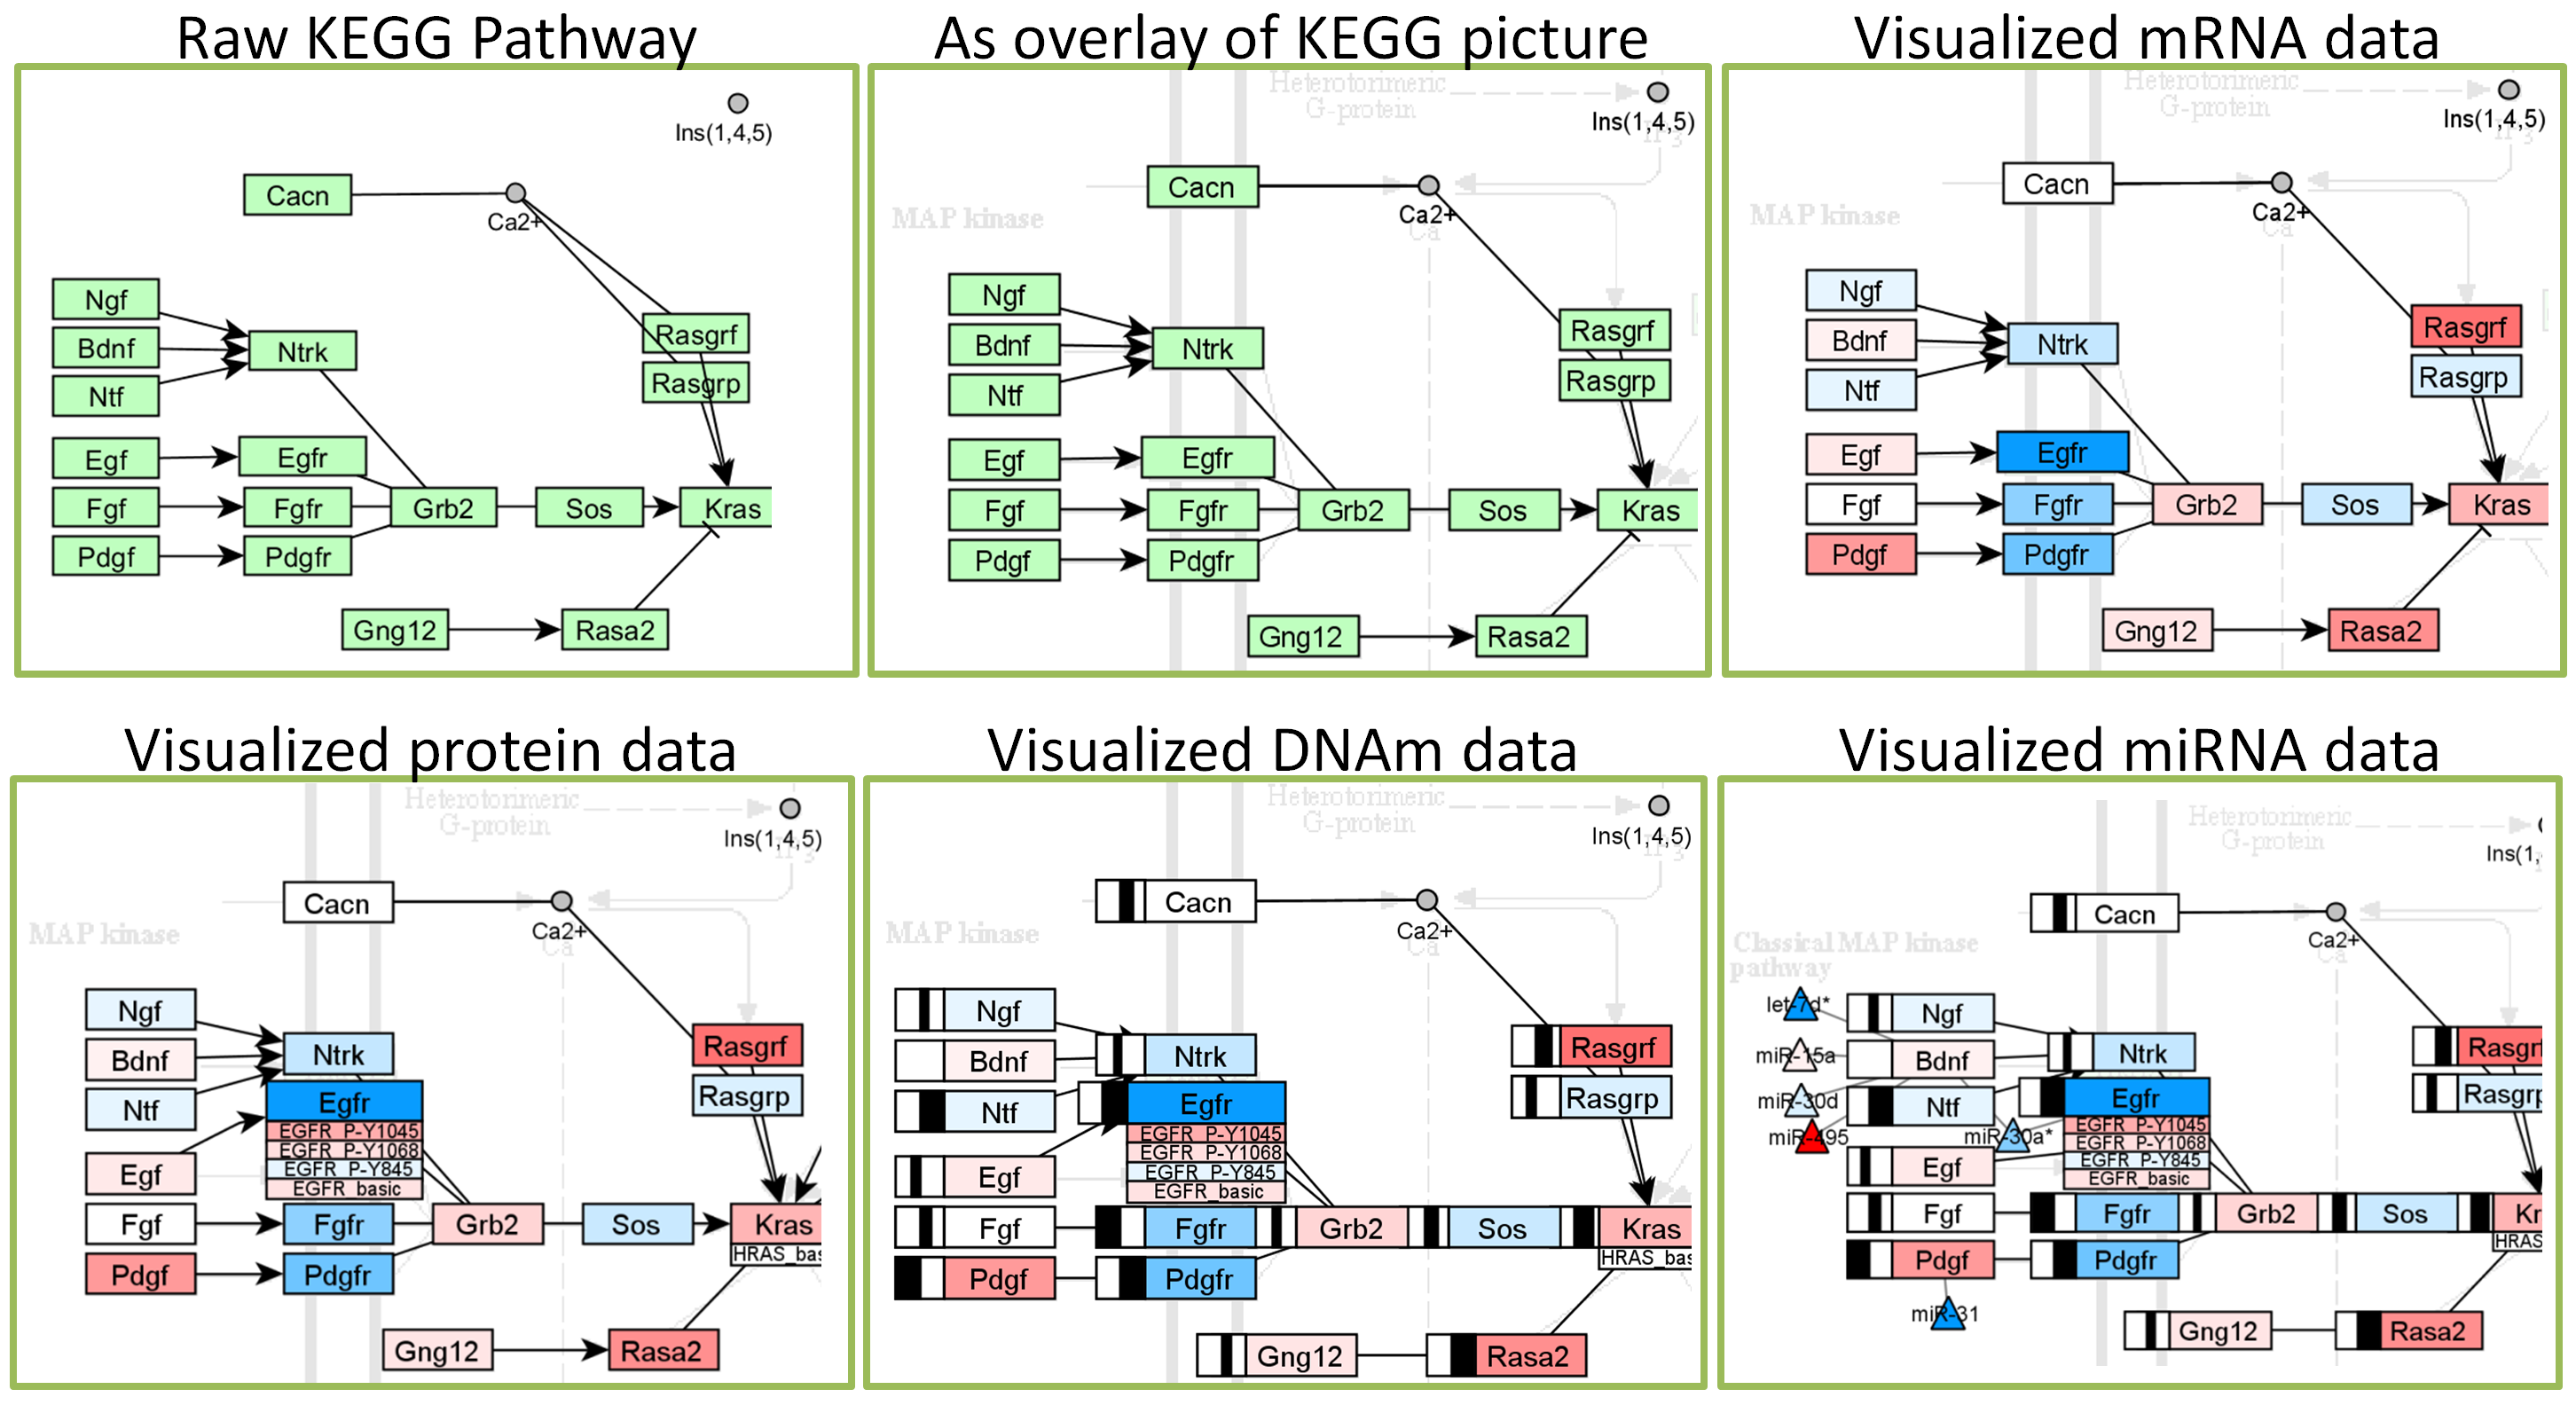
\includegraphics[width=1.0\textwidth]{figures/visualization-steps.png}
\caption{
TODO: Bild zeigt AUSSCHNITT des MAPK signaling pathway. Alle Schritte von a) bis f) kurz erlauetern und kurz sagen, dass f) quasi dem finalen Bild dieser Methode entspricht. }\label{fig:visualization_steps}
\end{figure*}


TODO:
 - Sollen wie noch "Table 1" aus MARCAR D4.1 reinnehmen (tabellarische erklaerung der visualisierung aller 4 datentypen mit beispielen), und/oder
 - Ein schoenes Gesamtbild e.g. von cell cycle oder wnt signaling oder sowas
[ - den metabolic pathway overview mit eingefarbten knoten] Dies nur wenn diese Methode auch noch bestandteil dieses papers wird (muesste noch bei methoden usw. aufgenommen und erklaert werden).


\section{Conclusion}

TODO: Zusammenfassung, vor allem Einzigartigkeit der Methode (insb. miRNA, (DNAm)) herausstellen, und kurze interpretation eines finalen bildes liefern ("man sieht in einem bild pathway informationen, miRNA relationen, expressionsdaten von miRNA, mRNA, bla; und sonst ist meist nach dem enrichment schluss bzw mRNA einfarbung bereits das maximum moegliche").



\section*{Acknowledgement}
We gratefully acknowledge contributions from Andreas Dr\"ager and Finja B\"uchel, as well as the whole MACRCAR consortium.

\paragraph{Funding\textcolon} The research leading to these results has received funding from the Innovative Medicine Initiative Joint Undertaking (IMI JU) under grant agreement nr. 115001 (MARCAR project).

\bibliographystyle{natbib}
%\bibliographystyle{achemnat}
%\bibliographystyle{plainnat}
%\bibliographystyle{abbrv}
%\bibliographystyle{bioinformatics}
%\bibliographystyle{plain}

\bibliography{document}
%TODO: When paper is ready, comment \bibliography line and add content of document.bbl here.

\end{document}
